\section{Проводимость полосы топологического изолятора
         в формализме Ландауэра--Буттикера}
Проводимость полосы можно вычислять в формализме Ландауэра--Буттикера, как
это делается, например, в \cite{Li2009}. А именно, для системы, состоящей
из полосы топологического изолятора и присоединённых к ней бесконечных
контактов, решается задача рассеяния. Проводимость даётся формулой
Ландауэра:
\begin{equation}
    G = \frac{2_se^2}{2\pi \hbar} \Tr{\hat{t}^\dagger \hat{t}}
\end{equation}
Здесь $\hat{t}$ --- матрица рассеяния из одного контакта в другой. 

Задача рассеяния в такой постановке может быть эффективно решена численно
(см. приложение~\ref{app:kwant}). Для этого существует библиотека Kwant 
\cite{Groth2014} для языка программирования Python.

Мы рассматривали контакты, описываемые гамильтонианом
\begin{equation}
    H_{\mathrm{Lead}} = \sum_i (E + 4t)c_{i}^\dagger a_{i} - \sum_{<i,j>} t c_{i}^\dagger c_{j}
\end{equation}
Они соединялись с топологическим изолятором посредством членов $c_i^\dagger a_{j,\sigma}$, 
где $c$ --- операторы контакта, а $a$ --- топологического изолятора.

В \cite{Li2009} (а также в многих других работах) исследуется зависимость проводимости 
бруска от беспорядка. Беспорядок реализовывался следующим образом:
к энергии каждого узла добавлялась случайная величина, равномерно распределённая в 
$[-W/2, W/2]$ ($W$ --- амплитуда беспорядка).При энергии, лежащей в щели, зависимость 
проводимости от амплитуды
беспорядка показана на рис.~\ref{fig:cond_vs_disorder}. Видно, что проводимость начинает 
уменьшаться только при очень большой амплитуде беспорядка,
сравнимой с характерной энергией связи между узлами. Однако в \cite{Li2009} не показано,
как отличается плотность состояний неупорядоченного топологического изолятора от идеального. 
Было бы логично предположить, что падение сопротивления начинается в тот момент, когда
из--за беспорядка появляется достаточное количество состояний в щели и происходит гибридизация
краевых состояний с примесными.

\begin{figure}[h]
    \centering
    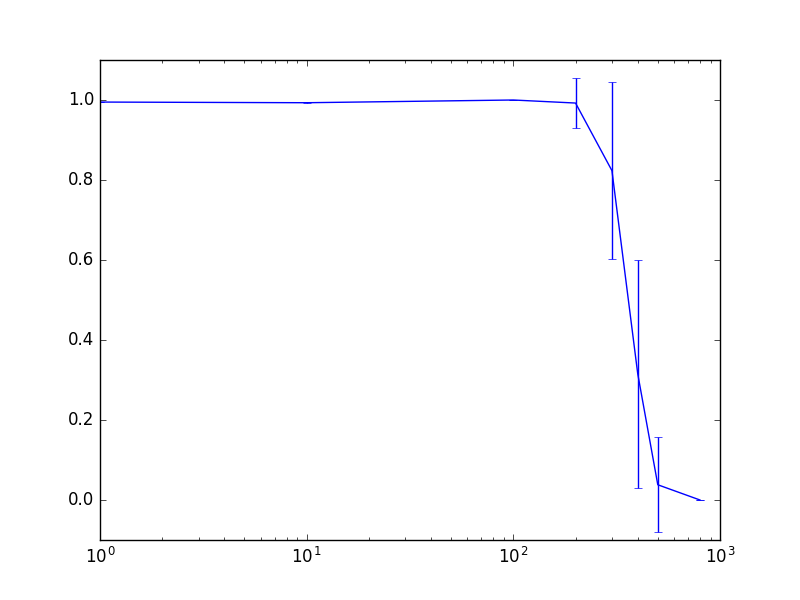
\includegraphics[width=0.5\linewidth]{cond_50x100_li2009.png}
    \caption{Зависимость проводимости полосы топологического изолятора от силы беспорядка}
    \label{fig:cond_vs_disorder}
\end{figure}


Мы провели аналогичные симуляции, одновременно вычисляя плотность состояний топологического
изолятора для различных амплитуд беспорядка. Кроме того, мы пробовали реализовывать 
беспорядок несколько по--другому. А именно, к каждому узлу с малой 
вероятностью $n$ добавлялась случайная величина, где $W$ с самого начала не мало. Это можно
интерпретировать как добавление небольшого количества примесей. Такой способ задания беспорядка
отличается от <<классического>> тем, что даже при малой концентрации примесей появляется
ненулевая плотность состояний внутри щели. 

Для различных реализаций беспорядка мы вычисляли зависимость проводимости от энергии Ферми, а
также плотность состояний с помощью прямой диагонализации. При отсутствии или малом значении 
беспорядка (или малой концентрации примесей) наблюдались 
чётко выраженные плато в зависимости проводимости от энергии.

Оказалось, что отсутствие щели в объёмной плотности состояний не обязательно приводит 
к исчезновению плато проводимости. Для <<обычного>> беспорядка плато исчезают
и сменяются хаотическими флуктуациями не в тот момент, когда исчезает щель, а при гораздо
более сильном беспорядке, когда близок к исчезновению минимум в плотности состояний,
соответствующий щели. Добавление малого количества <<глубоких>> примесей...
\begin{figure}[h]
    \centering
    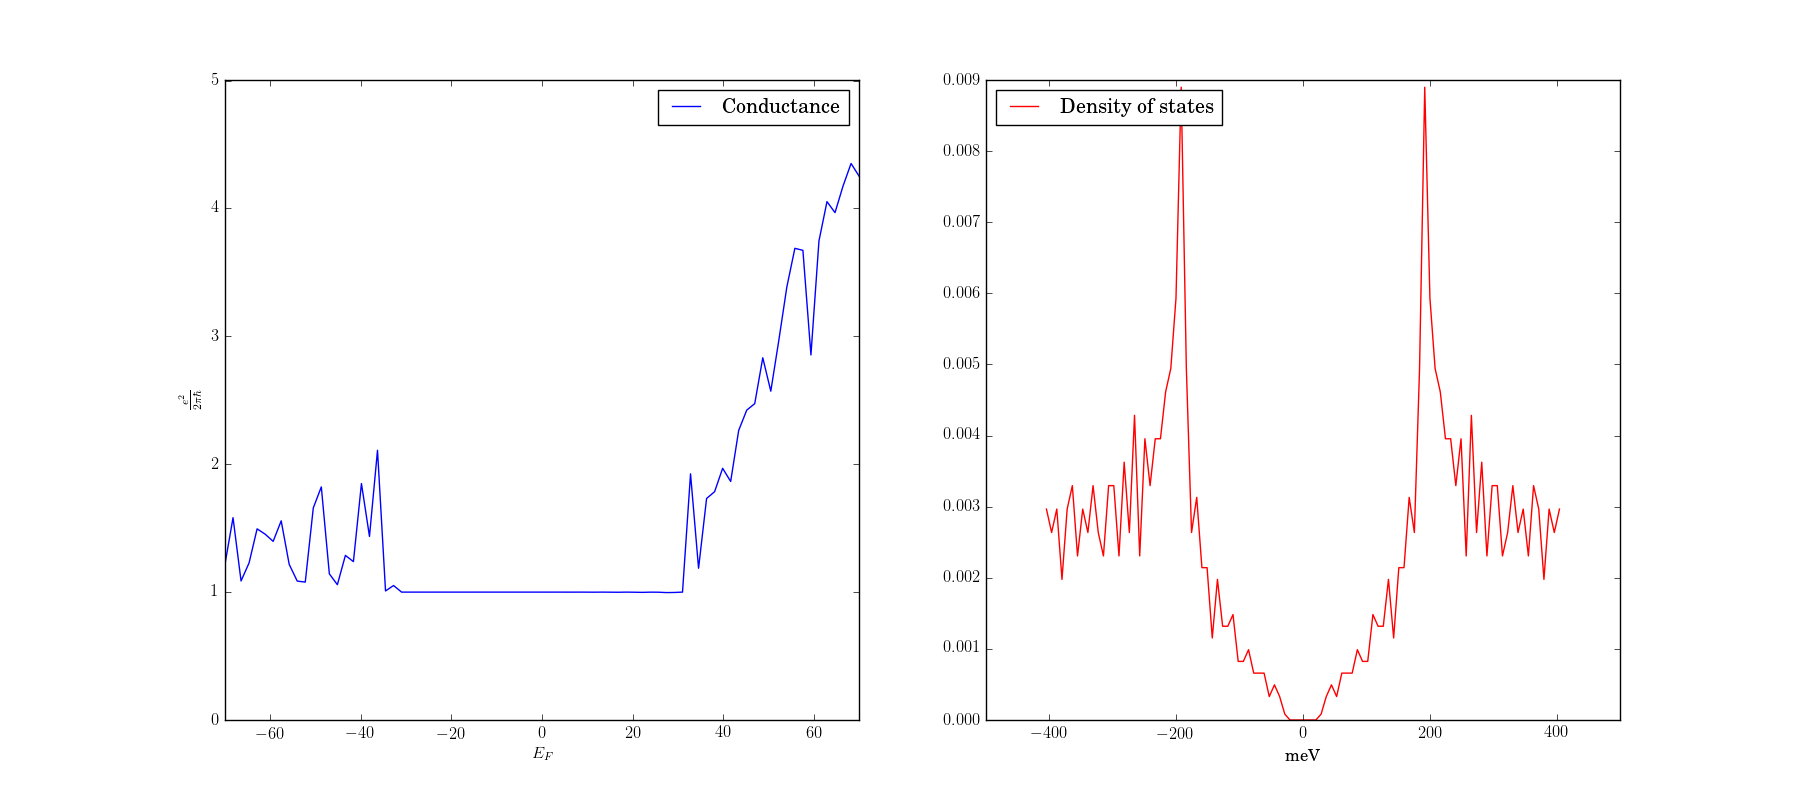
\includegraphics[width=0.9\linewidth]{dis_000.png}
    \caption{В отсутствие беспорядка 
             в щели наблюдается плато проводимости $G = \frac{e^2}{2\pi\hbar}$, 
             а плотность состояний равна нулю. 
             }
\end{figure}

\begin{figure}[h]
    \centering
    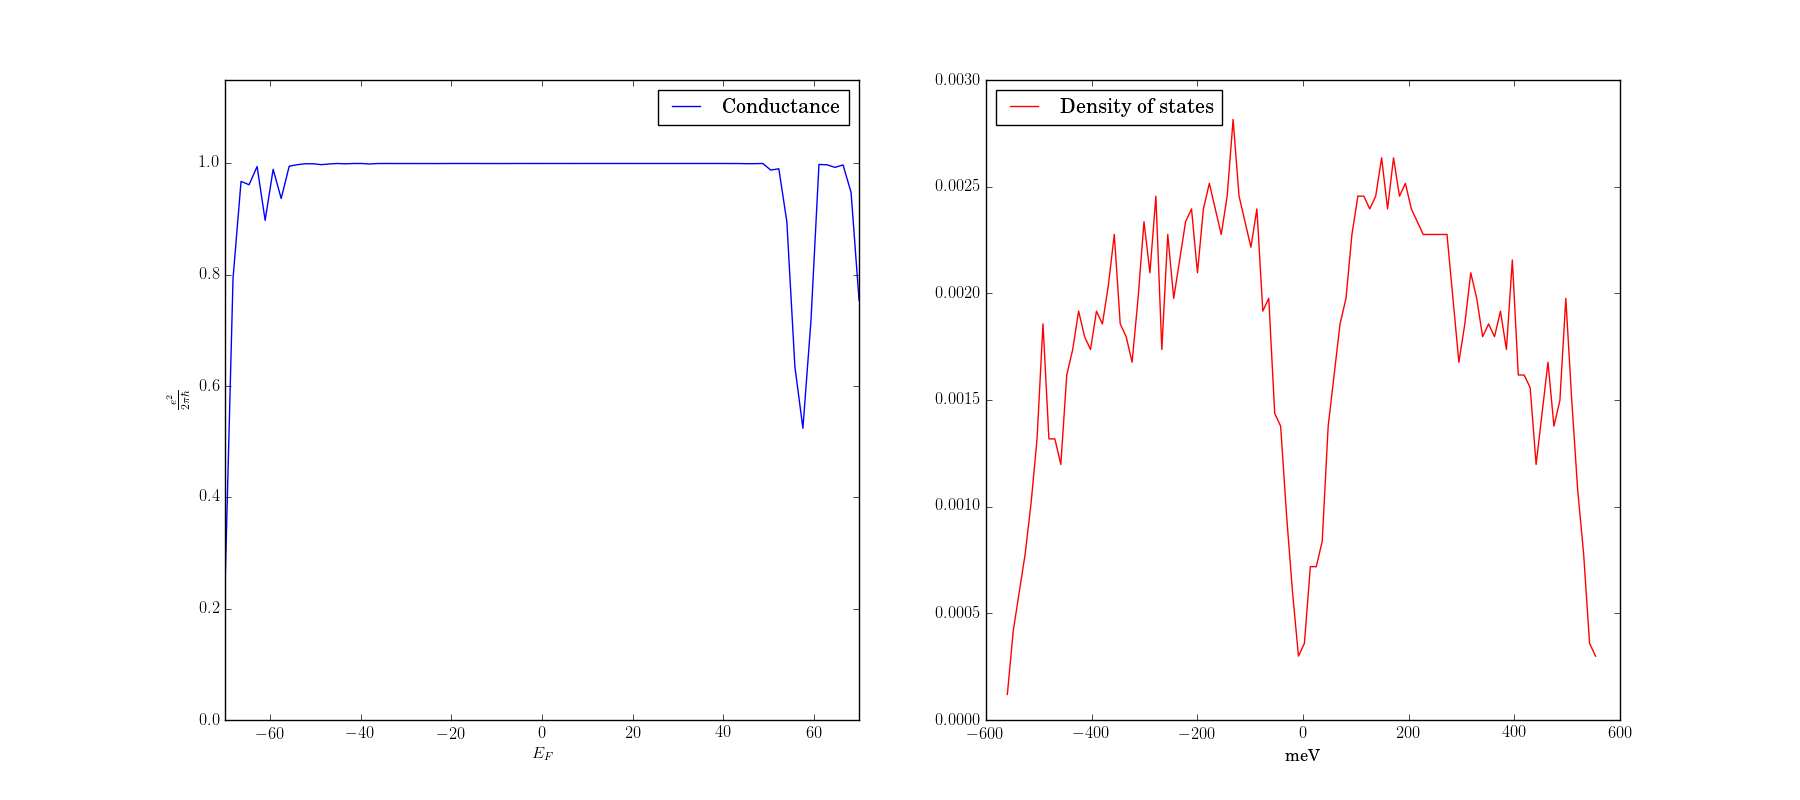
\includegraphics[width=0.9\linewidth]{dis_240.png}
    \caption{На данном рисунке сила беспорядка равна $240 \mathrm{meV}$. Видно, что плато 
             сохраняется, несмотря на ненулевую плотность состояний в щели.}
\end{figure}

\begin{figure}[h]
    \centering
    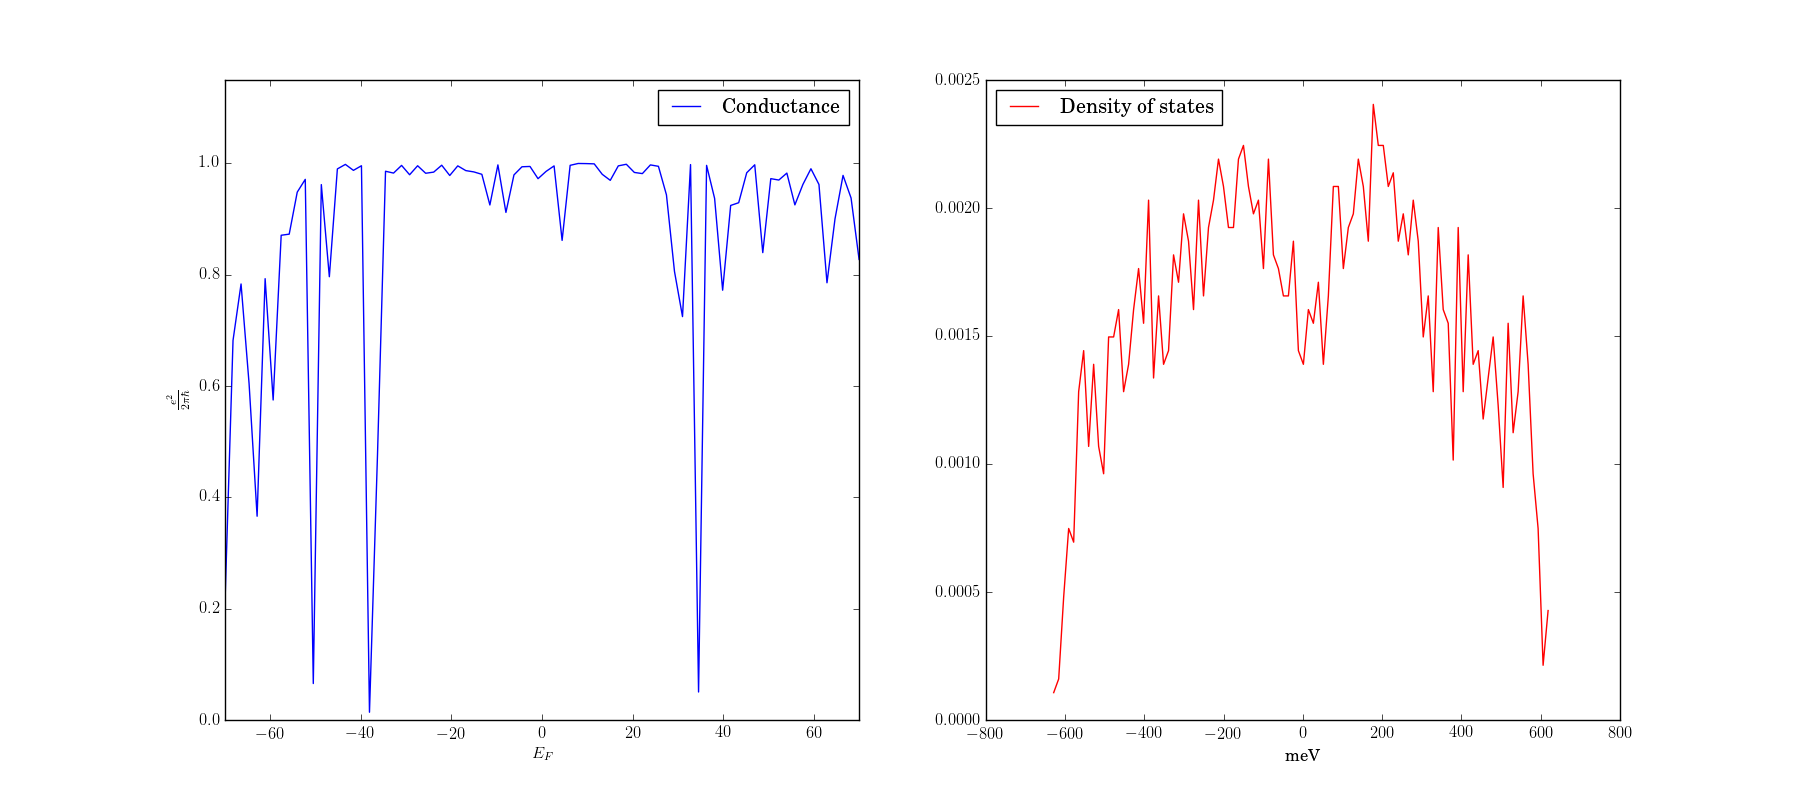
\includegraphics[width=0.9\linewidth]{dis_320.png}
    \caption{При ещё большей амплитуде беспорядка ($W = 320\mathrm{meV}$) проводимость начинает
             флуктуировать, но плато всё равно хорошо различимо. Дальнейшее увеличение $W$ 
             приводит к нарастанию флуктуаций, а в дальнейшем --- к исчезновению плато.}
\end{figure}

%\begin{figure}[h]
%    \centering
%    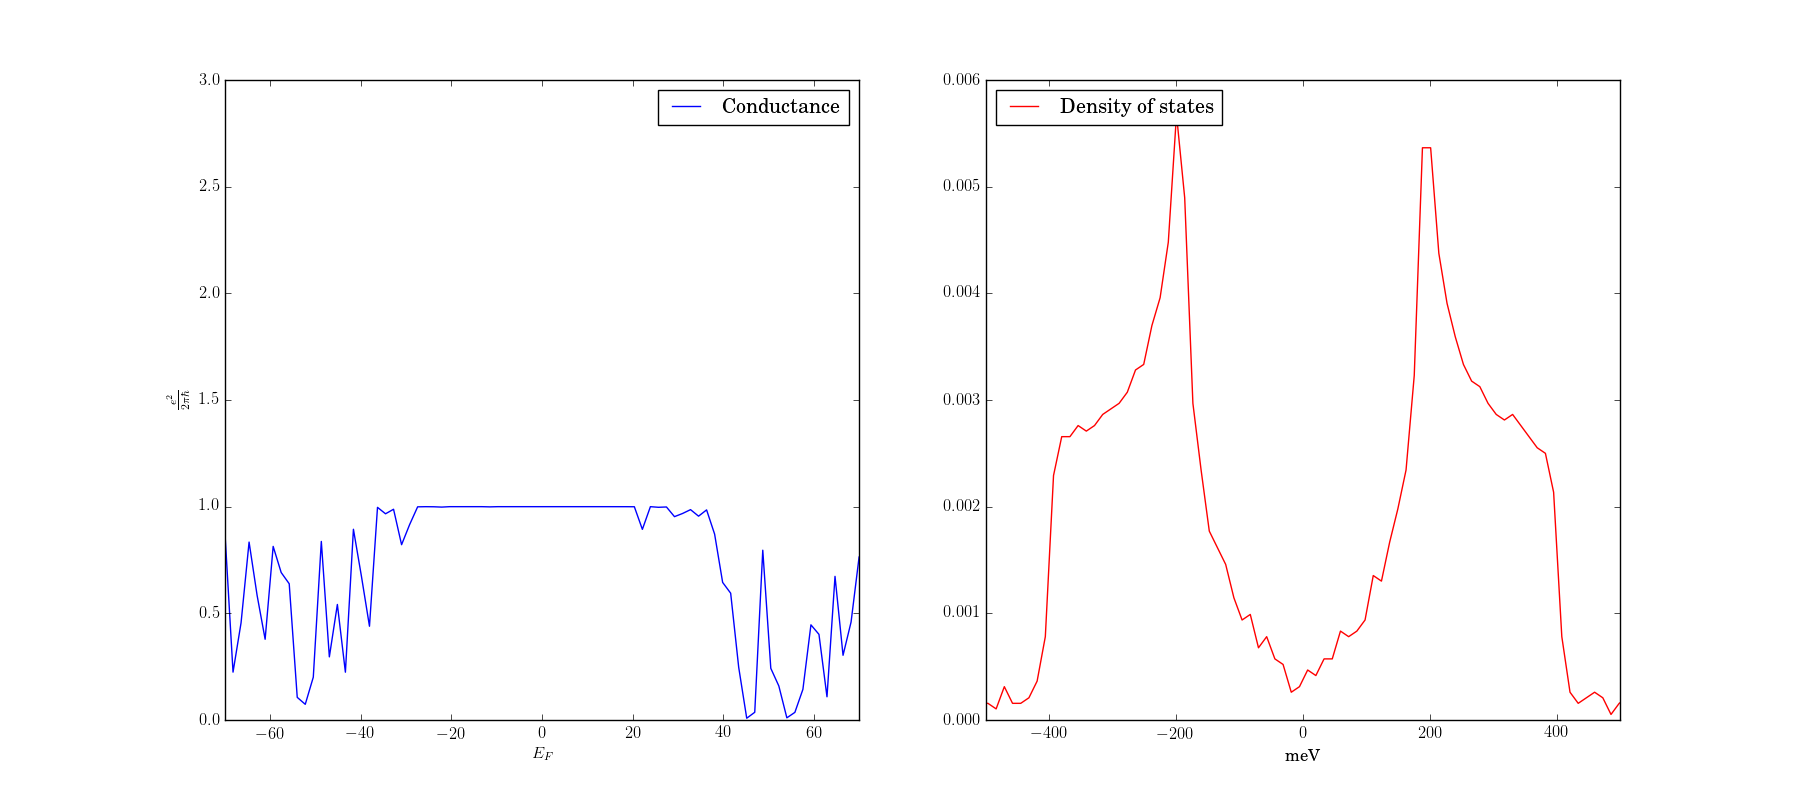
\includegraphics[width=0.9\linewidth]{prob_0-100.png}
%    \caption{Большая концентрация случайных глубоких примесей}
%\end{figure}
%
%\begin{figure}[h]
%    \centering
%    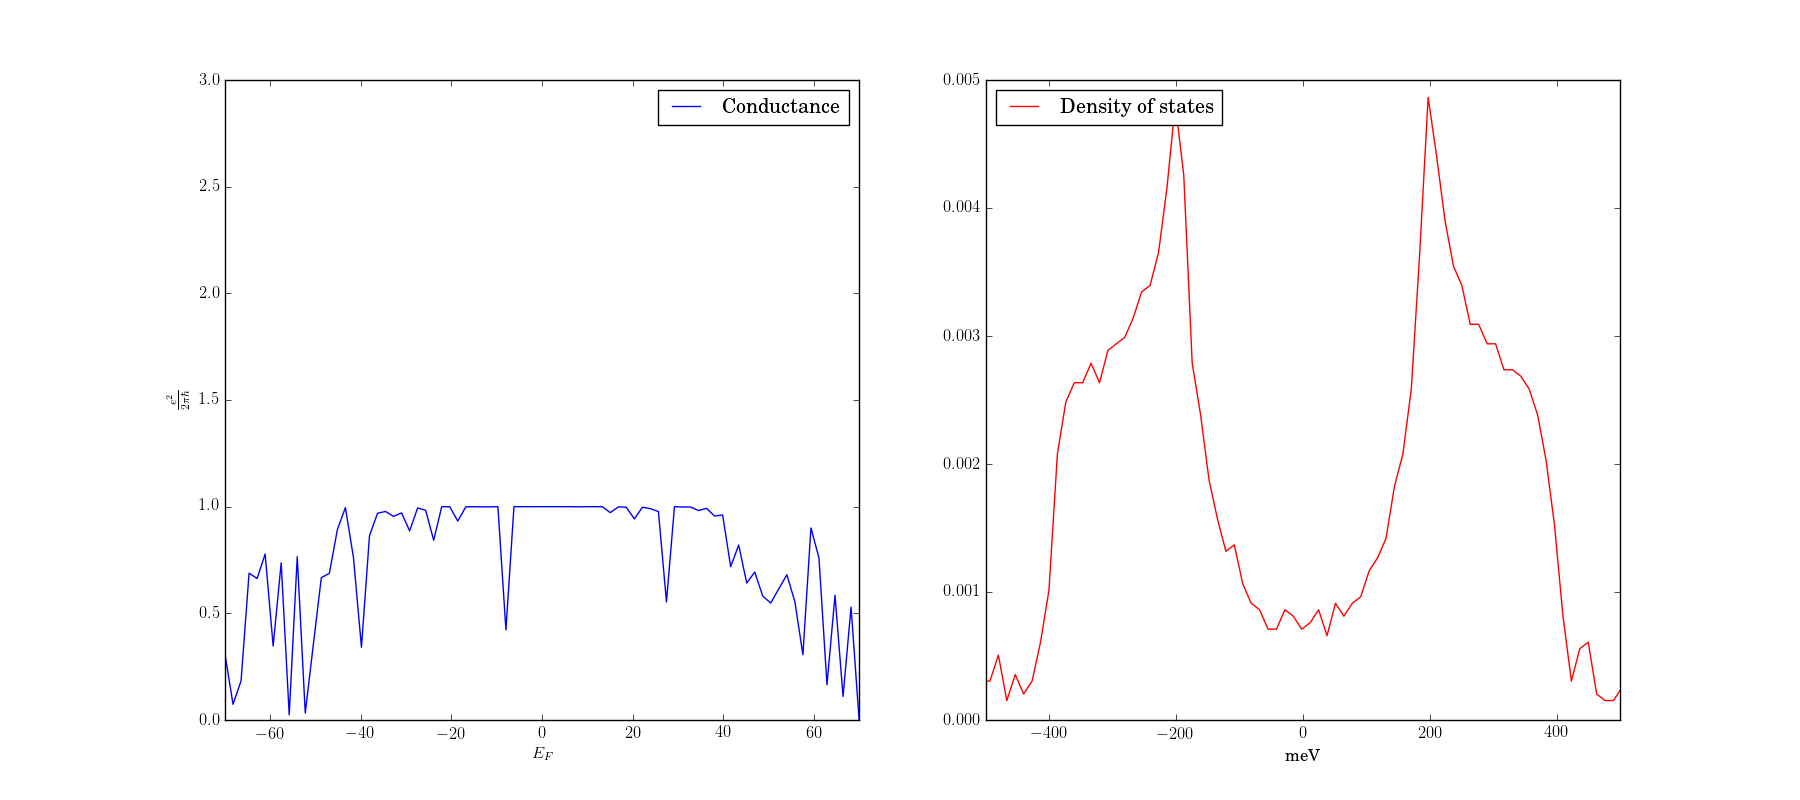
\includegraphics[width=0.9\linewidth]{prob_0-200.png}
%\end{figure}
\clearpage
